\section{Math}

The math for the wind simulation is based on the computational fluid dynamics
model described in the Background chapter. This model was included in the first 
snow simulator by Saltvik\cite{originalSnowThesis} and later in the GPU 
implementation by Eidissen\cite{gpuSnowThesis}.

In computational fluid dynamics, the Navier-Stokes equations are used to describe 
fluid flow. In the Background chapter this equation was reduced to the 
incompressible Euler equation by assuming zero viscosity and a density equal to 
one. Further more it is assumed that the contribution of external forces like 
gravity are negligible. In three dimensions, these assumptions leads to the 
following equations. 

\begin{equation} 
	\tag{momentum equation}
	\pOne{t}u(x, y, z) = -(u(x, y, z) \cdot \nabla)u(x, y, z) - \nabla p(x, y, z)
\end{equation}

\begin{equation}
	\tag{continuity equation}
	\nabla \cdot u(x, y, z) = 0
\end{equation}

$u(x, y, z)$ is the wind velocity field, a three dimensional field of three
dimensional velocity vectors. $p(x, y, z)$ is the pressure field, a three
dimensional field of scalar values. In the following derivations $u$ is short
hand notation for $u(x, y, z)$ and $p$ short hand for $p(u, x, y)$. The full
notation will only be used when writing down the final equations that will be 
used in the wind simulator.

The momentum equation is an expression for the change in velocity of the
fluid. Given an initial velocity $u_n$ at time $t_n$, we can compute the velocity 
$u_{n+1}$ at time $t_{n+1}$ with Euler integration.

$$ u_{n+1} = u_n + \pOne{t}u_n \delta t $$

Here $n$ is the time step and $\delta t$ is the time difference between time step 
$n$ and $n+1$. Plugging in the momentum equation leads to the following expression.

$$ u_{n+1} = u_n + \big( -(u_n \cdot \nabla)u_n - \nabla p_n \big) \delta t $$

$$ u_{n+1} = u_n - (u_n \cdot \nabla)u_n \delta t - \nabla p_n \delta t $$

By inserting this expression into the momentum equation we can derive the
expression for the pressure. 

$$ \nabla \cdot u_{n+1} = 0 $$

$$ \nabla \cdot u_n - \nabla \cdot (u_n \cdot \nabla)u_n \delta t - \nabla^2 p_n \delta t = 0 $$

The contribution from the term $ \nabla \cdot u_n $ is zero because of the continuity equation.

$$ \nabla^2 p_n \delta t = - \nabla \cdot (u_n \cdot \nabla)u_n \delta t $$

$$ \nabla^2 p_n = - \nabla \cdot (u_n \cdot \nabla)u_n $$

Using this equation for pressure ensures that the velocity field is divergence-free.

Calculating the velocity at time step $n+1$ requires three steps, advection, 
solving the Poisson equation, and projection.

\subsection{Advection}

Advection is the first term of the momentum equation, $-(u \cdot \nabla)u$, and
describes the fluid's ability to transport velocities along it's own velocity 
field. This step calculates a temporary velocity field that is required to solve
the Poisson equation for the pressure field.

$$ \nabla^2 p = - \nabla \cdot (u \cdot \nabla)u = \nabla \cdot u^* $$

When written out for each of the three dimensions for the wind simulation, the
equation becomes

$$ u^* = [u^*_x, u^*_y, u^*_z] $$
$$ u^*_x = - \Big( \pOneD{u_x^2}{x} + \pOneD{u_x u_y}{y} + \pOneD{u_x u_z}{z}\Big) $$
$$ u^*_y = - \Big( \pOneD{u_x u_y}{x} + \pOneD{u_y^2}{y} + \pOneD{u_y u_z}{z}\Big) $$
$$ u^*_z = - \Big( \pOneD{u_x u_z}{x} + \pOneD{u_y u_z}{y} + \pOneD{u_z^2}{z}\Big) $$

These partial differential equations can be approximated using a finite difference
approximation. However this method may be numerically unstable. Instead another
approach described by Saltvik\cite{originalSnowThesis} has been implemented.

The idea behind this approach is to model the fluid as a set of particles and to
trace the particles path through the velocity field. If $x$ is a cell in the
discrete grid, the velocity of the fluid in that cell is given by $u(x)$. The
velocity of the particle in cell $x$ is calculated by tracing the particle's path
backwards through the velocity field as illustrated in figure \ref{fig:backtrace}.

\begin{figure}[ht]
	\center
	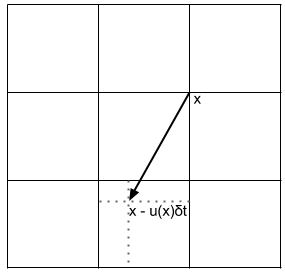
\includegraphics[width=0.5\textwidth]{images/advect_back_trace}
	\caption{On grid velocities are traced backwards in time.}
	\label{fig:backtrace}
\end{figure}

$$ u^*(x) = u(x - u(x) \delta t) $$

The velocity value at $ x - u(x) \delta t $ is interpolated from the nearest
grid cells. This method is only stable if the time step is small enough, 
otherwise several grid cells can be jumped over when tracing the particle's
path. 

\subsection{Poisson equation}

The Poisson equation has to be solved to get the value of the pressure field. 

$$ \nabla^2 p = \nabla \cdot u^* $$

This equation is solved numerically using the finite difference approximation
introduced in the Background chapter. The Poisson equation can be rewritten as 
a system of linear equations on the following form.

$$ Ap = b $$

Here $A$ is a matrix, $p$ is the pressure field represented as a vector and $b$
is a vector calculated from $\nabla \cdot u^*$. The Poisson equation is discretized 
by sampling the problem domain in $n_x+1$ points in the $x$ dimension, $n_y+1$
points in the $y$ dimension and $n_z+1$ points in the $z$ dimension. The sample
points on the border of the domain are boundary points that have their values
specified by the boundary conditions of the problem. The boundary conditions
are discussed later. This means that the number of internal points, or degrees of
freedom, is $N = (n_x-1) \cdot (n_y-1) \cdot (n_z-1)$. The step length between 
each sample point in the x, y and z dimension is given by 

$$ h_x = \frac{1}{n_x}, ~ h_y = \frac{1}{n_y}, ~ h_z = \frac{1}{n_z} $$

For brevity's sake, $p_{i, j, k}$ is used as shorthand notation for 
$p(ih_x, jh_y, kh_z)$. $u^*_{i, j, k}$ is used as shorthand notation for
$u^*(ih_x, jh_y, kh_z)$.

\subsubsection{Linear System}

When written out for three dimensions, the expression for the Poisson equation
becomes

$$ \pTwoD{p}{x} + \pTwoD{p}{y} + \pTwoD{p}{z} = \pOneD{u^*_x}{x} + \pOneD{u^*_y}{y} + \pOneD{u^*_z}{z} $$

This equation is then discretized using the finite difference method described
in the Background chapter. For the left hand side the approximation derived for 
the second derivative is used.

$$ \pTwoD{p}{x} = \frac{p_{i+1, j, k} - 2p_{i, j, k} + p_{i-1, j, k}}{h_x^2} $$
$$ \pTwoD{p}{y} = \frac{p_{i, j+1, k} - 2p_{i, j, k} + p_{i, j-1, k}}{h_y^2} $$
$$ \pTwoD{p}{z} = \frac{p_{i, j, k+1} - 2p_{i, j, k} + p_{i, j, k+1}}{h_z^2} $$

For the right hand side the central difference approximation is used.

$$ \pOneD{u^*_x}{x} = \frac{(u^*_{i+1, j, k})_x - (u^*_{i-1, j, k})_x}{2h_x} $$
$$ \pOneD{u^*_y}{y} = \frac{(u^*_{i, j+1, k})_y - (u^*_{i, j-1, k})_y}{2h_y} $$
$$ \pOneD{u^*_z}{z} = \frac{(u^*_{i, j, k+1})_z - (u^*_{i, j, k-1})_z}{2h_z} $$

\subsection{Projection}

Using the pressure field calculated earlier we calculate the final term of the 
momentum equation, $-\nabla p$. The gradient of the pressure field is discretized 
using the central difference approximation to approximate the partial derivatives.

$$ (-\nabla p)_{i,j,k} = -\Big( \pOneD{p_{i,j,k}}{x}, \pOneD{p_{i,j,k}}{y}, \pOneD{p_{i,j,k}}{z} \Big) $$

$$ \pOneD{p_{i,j,k}}{x} = \frac{p_{i+1,j,k} - p_{i-1,j,k}}{2h_x} $$
$$ \pOneD{p_{i,j,k}}{y} = \frac{p_{i,j+1,k} - p_{i,j-1,k}}{2h_y} $$
$$ \pOneD{p_{i,j,k}}{z} = \frac{p_{i,j,k+1} - p_{i,j,k-1}}{2h_z} $$

With this the final expression for the next wind velocity becomes

$$ u_{n+1} = u_n - u^* \delta t - \nabla p \delta t $$

where $u^*$ is calculated in the advection step and $p$ is calculated by solving
the Poisson equation. $u_{n+1}$ is the updated wind velocity and $u_n$ is the
wind velocity from the previous time step.

\subsection{Boundary Conditions}

For the purpose of the wind simulation the wind velocity on the boundary of the
domain is set to some constant values set by the user. This means that the flow
into and out of the domain defines the velocity field, except for on the border
of the terrain where the wind velocity normal to the boundary is set to 0.

The boundary conditions were specified the same way as in Saltvik's paper
\cite{originalSnowThesis}, where the boundary conditions are based 
on the method from Realistic Modelling of Falling and Accumulating Snow, a master
thesis by Aagaard et al\cite{danishSnowThesis}. 

For the pressure field Neumann boundary conditions are used. This means that
the normal pressure gradient along the boundary is 0. This is done by setting
the pressure on the boundary to be equal to the pressure on the inside of the 
boundary.
